%Chapter 3
\chapter{Theoretical Analysis and Approach}
\label{chap:analysis-and-arch}
This chapter presents an analysis of the system and literature regarding previous research.
It will segment different subsystems to separate the controlled system, the engineered system and the environment they are deployed in.
With the analysis done, we will have a clear understanding of relevant parameters and their interaction.
Which will be the basis for a sensitivity analysis to determine the most impactful components.
From this the main goal of this work is extracted.
Knowing the objective and the most influential elements enables us to map out a solution proposal.
It also prepares us for the simulation brought fourth in chapter \ref{chap:simulation}.

First introduce the system and what is important, so the reader understands current implementations.
Then prune the system to sculpt our concept.
% We will first discuss the general concept to unde

% This chapter will give an overview over the state-of-the-art research.
% It examines the impact of 

% This chapter shall define the system and its boundaries.
% Define the goal of this work.
% This chapter will uncover the problem we are trying to solve.
% What it is we are trying to achieve.
% Then analysis of state of the art solutions.
%
\section{System Analysis}
\label{sec:system-analysis}
To design a solution, we must first know the structure of the problem. %and establish some terminology.
For this we need to get a tangible definition of the term system.
% For this we need to get more tangible with the term system.
% To break down, we must first know what a system is.
% A system might be defined in different ways.
% There exist different definitions of a system.
% There exist different definitions for what a system is.
For the engineer, it can be described as a collection of elements with properties of interest @schmitt2019.
Following this definition, we need to identify the systems' constituents.
And then analyze what about them is important to us.
% So let us first break down the different parts.
The next section will break down the different parts.
% When we have an overview, we review existing systems.
% So what are the constituents, and which attributes need to considered?
% We will define this by the necessary functions which a system like this needs to fulfill.

\subsection{Partitioning}
\label{sub:partitioning}
The primary classification is to distinguish between controlled system, engineered system and context.
The plant is the basis of the \textit{Controlled System}.
However, it is not possible to manage it directly.
% It can only be placed into an environment which 
We need to interface with its environment to affect these green lifeforms.
This environment is further divided into leaf and root surroundings, since they require different conditions.
Apparent from their different situation in nature.

Going back to the fundamentals of \ac{cea}, the \textit{Engineered System} is composed of three parts.
Illumination, irrigation and the atmosphere control.
They cater to the different needs of the plant.
Atmosphere control and illumination interface with the leaf environment, while irrigation takes care of the root system.
Together the controlled system and the engineered system make up, what we will call a 'farm'.

These parts are embedded into a greater \textit{Context} they need to operate in.
This is where this work diverges from previous concepts.
In the past, the field has tried to shield the farming context from outside influences.
Less exchange to the environment means a very high level of consistency and independence.
As we will see in the analysis of commercial farms (\ref{par:prop-ener-commercialfarms}), this approach has not proven successful though.
This is why this work embraces the context it operates in.
Seeing it not as a hindrance but as an opportunity for synergy.
As introduced before, this work places the farm on building facades. % we want to green facades.
Two different domains reveal themselves in this context.
The building insides and the city environment.
The \textit{City} in this work is classified as everything surrounding the envelope of the farm.
Therefore, the outside world with weather and the suns' radiation is integrated here and enables a hybrid approach to plant cultivation.
Part utilization of natural resources and part artificial optimization of the environment.
Similar to how greenhouses operate already. 
The interface to the \textit{Building} is novel. %directly leads to insulation
Potential for insulation naturally comes to mind, which provides a big benefit not exhausted in this work.
We will only evaluate insulation performance.
Energy savings for the building brought about by this choice are not considered in the energy balance built up in later chapters.
 % but not yet add it to the energy savings achieved by our design.
% Only skimmed by evaluating insulation performance but not exhaustivily discussed.
% The energy savings are not even considered.
% The possibility of building insulation emerges naturally by this.

These are the general parts which comprise our concept.
In the next section we will delve deeper into their interactions.
They will make up the properties of interest which are still missing for our system definition (\ref{sec:system-analysis}).

\subsection{Properties of Interest}
\label{sub:prop-of-interest}

\subsubsection{Controlled System}
\begin{wrapfigure}{R}{0.4\textwidth}
	\caption{The plant and its immediate environment.}
	\label{wfig:controlled-system}
	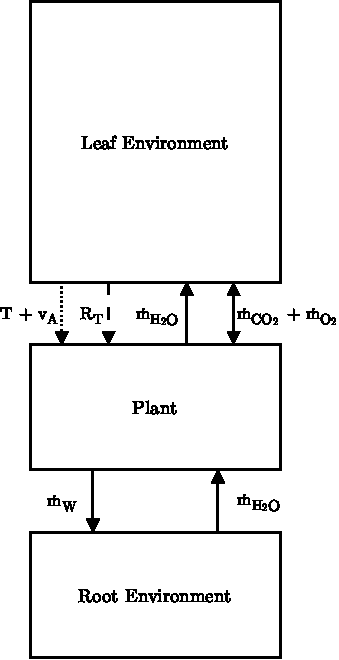
\includegraphics[width=0.4\textwidth]{img/controlled-system.pdf}
\end{wrapfigure} 

Beginning with the system we want to control, we illuminate the interface between the plant and its environment.
The root system is relatively straight forward to manage.
We need to supply water and nutrients while cleaning out waste products.
These are modeled as mass flows.
Water and substances dissolved within it are named $\dot{m}_{\text{H}_2\text{O}}$ in this work.
The waste products are captured with $\dot{m}_\text{W}$.

Shifting up to the leaf environment, photosynthesis presupposes two mass flows as well.
Carbon dioxide $\dot{m}_{\text{CO}_2}$ moves from the air to the leaves, while oxygen $\dot{m}_{\text{O}_2}$ diffuses out to the atmosphere.
During nighttime these flows are reversed to accommodate cellular respiration.
This is however not everything happening at this interface.
Most of the water taken up by the roots is actually not used in photosynthesis at all.
The plant uses it to carry nutrients up into its body.
This movement is fueled by transpiration.
About \SI{95}{\percent} of the $\text{H}_2\text{O}$ is carried out to the environment this way \textcolor{Blue}{needs ref}.

Next, energy in the form of radiation is required.
The total radiation hitting the leave surface is characterized by $R_\text{T}$.
This incorporates the spectrum and intensity of the light.
% Depending on the source it is divided into \ac{par} and \ac{ppfd}.
With this we have captured properties which flow from one system to another in the targeted context.
% There is however also an informational
These are however not the only attributes of interest.

As shown later in the \nameref{subsub:yield-analysis} there are two other features of the atmosphere we need to take a closer look at.
Air temperature $T$ and air speed $v_\text{A}$.
These are inputs to the yield model we will introduce in the \nameref{subsub:yield-analysis}.
They are not flowing from one system to the other in a physical sense. % in contrast to the other characteristics.
Instead, these are properties informational in nature.
A block diagram of the plant and its immediate environment can be seen in figure \ref{wfig:controlled-system}.
Mass flows are shown as solid lines, energy fluxes dashed and data flow as dotted lines.
Now that we have defined the objective of our inquiry, the next section will talk about its supervision.

% \paragraph{}
% \vspace*{-\parskip}

\subsubsection{Engineered System}
\label{subsub:engineered-system}
% The first part we can influence, is
\begin{wrapfigure}{R}{0.6\textwidth}
	\caption{The technical system and its influences.}
	\label{wfig:engineered-system}
	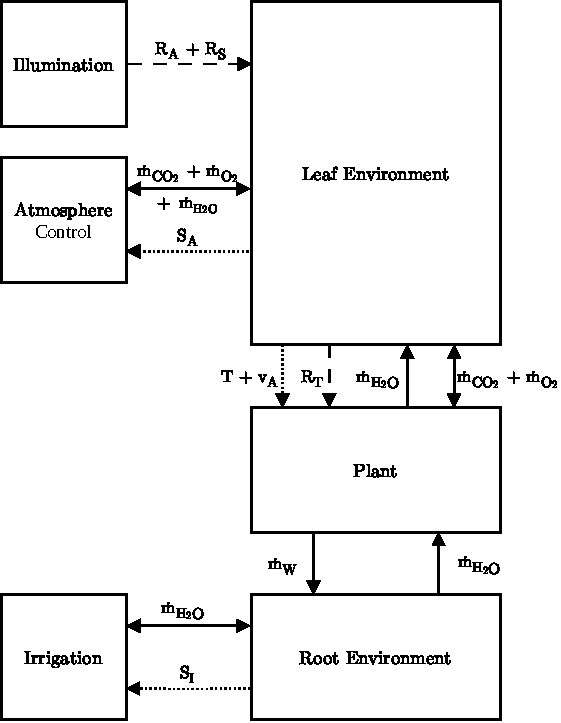
\includegraphics[width=0.6\textwidth]{img/engineered-system.pdf}
\end{wrapfigure} 

Following the partitioning, the first technical subsystem is illumination.
At first thought it seems like we can interface with the plant leaf directly here.
However, we only supply a certain \ac{par} / \ac{ppfd} to the environment.
The plant is free to use any amount of it and will actually close its stomata -- the pores enabling gas exchange -- in light stress situations \textcolor{Blue}{needs ref}.
Effectively caping the light it uses.
And so the artificial radiation $R_\text{A}$ flows from the light source to the leaf environment.
Another influence we can take on lighting is to shade the plants from excessive natural lighting.
This is frequently done in existing greenhouses to prevent aforementioned light stress.
The amount of light passing through will be called $R_\text{S}$.
This can be unimpeded or diffused natural radiation by shading.

Next let us look at atmosphere control.
\textcolor{Blue}{Heat flow to heat or cool the air volume is missing.}
\textcolor{Blue}{Heat output from LEDs missing.}
The mass flows $\dot{m}_{\text{H}_2\text{O}}$, $\dot{m}_{\text{CO}_2}$ and $\dot{m}_{\text{O}_2}$ introduced before can all be controlled discretely.
Water in the form of humidity is an important factor to control \ac{vpd} as introduced in the \nameref{sec:fund-cea}.
And elevated levels of carbon dioxide promote mass accumulation and therefore higher yields.
Oxygen is nonessential in our inquiry and is only distinguished to keep an equilibrium of elements in the leaf environment.
% Oxygen is not of big interest and is only distinguished 
% shown separately because of the importance of carbon dioxide and water.
For the control to function there needs to be some form of feedback.
Sensors to capture the relevant properties temperature, air speed and mass concentrations for water and CO$_2$ are placed in the air volume.
Note that carbon dioxide is usually measured as a volume concentration.
But, it is easy to convert these two values via the density.
And so no distinction is made in this investigation.
% For our investigation it is more convenient to look at mass flows.
% These values can be converted via the density.
Water in the form of humidity can be measured both as a mass or volume concentration.
The sensor data is aggregated with the atmosphere control signal $S_\text{A}$.

% For irrigation, we describe the water flow with any dissolved materials and waste products as $\dot{m}_{\text{H}_2\text{O}}$.
For irrigation, we describe the water flow with any dissolved materials as $\dot{m}_{\text{H}_2\text{O}}$.
Different to the water mass flow from the root zone towards the plant, this includes the waste products.
This is because at this point the pure waste products of the plants will be dissolved and transported together with the water flow.
\ac{vpd} of the root control volume is fed back through the irrigation control signal $S_\text{I}$.
With this we have gathered an overview of the attributes needed to govern the controlled system.
Figure \ref{wfig:engineered-system} shows the influences the technical system takes on the controlled system.
Subsequently, the next section introduces the setting in which this system is placed.
% will highlight the context of our system.

% Now we introduce the part we as an engineer have control over.
% On cloudy days, supplemental lighting.
% This artificial radiation is called $R_\text{A}$.
% Just as the natural radiation it captures spectrum and intensity.

% \paragraph{}
% \vspace*{-\parskip}

\subsubsection{Context}
As established before we divide the context into two domains.
First we examine the urban environment.
Natural radiation $R_\text{N}$ by the sun illuminates the city and therefore the farm.
We discussed before that this can be managed to a certain degree by shading our leaf environment.
So this illumination from the city domain interfaces with the corresponding control system.
% diffusing the incoming light.
% the illumination control by shading.
We still need an input signal for the light management.
It makes sense to choose the incoming illumination flux as our radiation control signal $S_\text{R}$.
Since it determines how much shade or supplemental light is needed.
Next the atmosphere control can interface with the city environment by exchanging air $\dot{m}_{\text{Air}}$.
This can be in the form of opening windows or a more complex interaction when processing air with \ac{hvac} units.
% Heat flow from the farm envelope to the environment or vice versa is not something we can actively control.
Apart from the material choices, heat transfer from the farm to the outside $\dot{Q}_{\text{FO}}$ is not something we can actively control.
And so it is shown as an energy flux between the building and leaf environments.
Note that the name $\dot{Q}_{\text{FO}}$ does not imply a direction of flow.
This is already taken care of by the direction of the arrows.
Other than introduced in the fundamentals on \nameref{sub:heat-transfer}, $\dot{Q}$ only includes conduction and convection.
Radiation is separated from the other heat transfers because it is special in our application and already modeled with $R_\text{N}$.

The important interaction taking place between the farm and the building interior is also a heat transfer $\dot{Q}_{\text{FB}}$.
The full block diagram of the system can be seen in figure \ref{fig:system-definition}.
This gives a good overview of what parts and properties are interesting when designing a concept for this application.
However, interest does not automatically imply necessity.
Fully controlled systems struggle to be profitable as teased before.
% A fully controlled system is not what this work is after as this has failed in the past.
Engineering is oftentimes about making compromises, so we have to analyze which features of the system are the most relevant.
This will enable us to make the right concessions and focus on the most impactful characteristics.
% This will enable to put the focus on the most impactful ones.
These themes are the topic of the next section.

\begin{figure}[htbp]
  \centering
  \caption{System partitioning and important flows.}
  \label{fig:system-definition}
  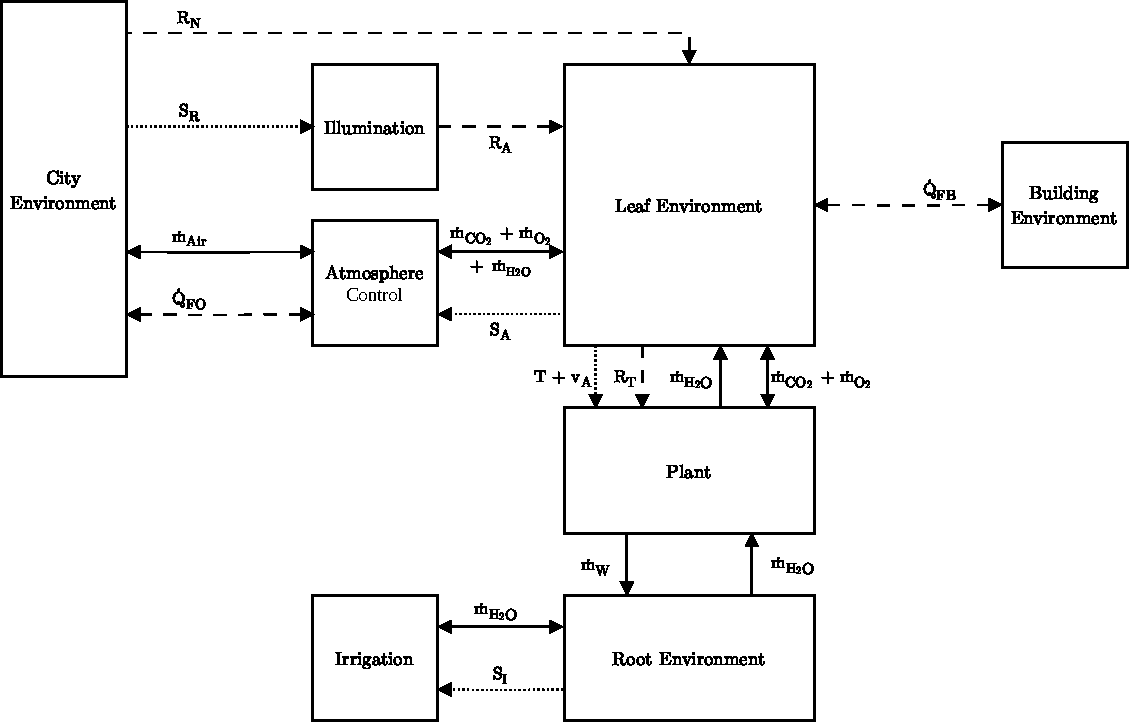
\includegraphics[width=\textwidth]{img/context.pdf}
\end{figure}

\subsection{Sensitivity}
The first part of this section will establish why the energy demand is an important attribute in this endeavor.
Then it will go deeper into which systems are the culprits for high power draw.
From this we will then formalize the main goal of this work, which is to minimize energy consumption.
Next the sensitivity of parameters influencing yield will be discussed.
This provides an understanding on which compromises are the least harmful to economic performance of the farm.
This constrains the main goal with an auxiliary condition.
Maximizing yield.
In the end this analysis lays the foundation on the choice of which parameters are free design variables.
And which are restricted by the application.

% The weight of the different properties are discussed in this chapter.

% Analyzing the important attributes will give us a clear view which parameters are free design variables.
% And which are constraint by other properties.

% This information is extracted from the objectives this work tries to optimize.
% Minimizing energy consumption and maximizing yield.
% \begin{itemize}
% 	\item Minimize energy consumption
% 	% \item Provide insulation
% 	% \item [Auxiliary condition] Maximize yield
% 	\item Maximize yield
% \end{itemize}
% These two goals are subjected to a sensitivity analysis in the following sections.
% This enables us to gain an understanding which parameters of the system are the most relevant.
% This helps us to identify the most relevant parameters.

% What elements have the biggest contribution to energy consumption?
% And what is the sensitivity of the elements to the yield output?
% Insulation will be evaluated but is no main design priority.
% There are elements consumed by the plant -- co2, water, light energy -- and there are ambient factors like air temperature and velocity.

\subsubsection{Energy Analysis}
\label{subsub:energy-analysis}
% Firstly this work looks into the state of existing commercial farms.
% This provides reason to divert from the current path the industry is taking.

% To be able to evaluate the energy impact of the different technical subsystems, we will look at current vertical farming system.

% Let us first examine current \ac{cea} and vertical farming approaches to get a better understanding of the solution methods and shortcomings.
% Current solutions try to achieve high degree of automation and full control over the environment.
% This results in high energy

% Companies such as ... and ... try to seperate the plants completely from the elements and control the environment they are in fully.
% This of course is great for reproducibility and quality.
% However as we will show later in chapter \ref{chap:analysis-and-arch} current commercially operating farms with this approch have one main problem.
% Energy consumption.

\paragraph{Commercial Farms}
\label{par:prop-ener-commercialfarms}
In recent years, hype surrounding vertical farming has slowed significantly.
2023 marked a \SI{91}{\percent} decrease in capital investment compared to the year before, according to Pitchbook.
% https://foodinstitute.com/focus/what-does-aerofarms-bankruptcy-signal-for-ceas-future/
Multiple commercial endeavors declared bankruptcy.
\textcolor{Blue}{How do I cite recent developments? Like companies going out of business?}
Especially in Europe where Energy prices surged in the last years.
One notable example is InFarm -- a Berlin startup which was able to gather significant funding.
Despite the financial backing, all European branches have seized operation.
They restructured and continue to function in the Middle East, where energy is less of a concern than water scarcity.
% They continue to function in the Middle East, but European branches have seized operation.
The company itself has cited high cost from energy consumption as the primary reason.
% https://www.infarm.com/news/note-from-infarm-s-founders-strategy-shift-and-profitability-at-infarm
A focus of the company was to diversify the crops which can be cultivated.
Exemplified by their efforts to grow wheat, a plant which has not been demonstrated in this setting before.

Aerofarms is another big player which recently filed for bankruptcy.
During this process they needed to refocus their efforts on their only profitable farm.
% They operate in the US and during this process needed to focus their efforts on only profitable farm.
% https://www.aerofarms.com/aerofarms-emerges-fully-funded-from-chapter-11/
% https://en.wikipedia.org/wiki/Controlled-environment_agriculture
% In general two trends are observable.
Both companies focused on a highly controlled and automated approach to farming.
This of course is great for reproducibility and quality.
But as happens frequently, tech companies want to optimize.
And since each plant can have drastically different requirements on the optimal condition, they invested heavily into R\&D.
Some amount of research is undoubtedly required to compete with traditional agriculture.
However, optimization is endless and only offers diminishing returns the further it goes.
It is easy to end up with an overengineered system.
% However, since most of the entrepreneurs in this field come from a tech background, they tend to
% But easily leads to overengineered systems.
The author of this work is a proponent of \acs{kiss} principles.
And so the most impactful factors should be considered first.
% Luckily nature mostly provides a non-hostile environment.
Nature is utilized to nurture the parts deemed less important.
% High investment cost and R\&D efforts are needed to compete

% The lessons which can be drawn from the abovementioned developments are as follows.
From the examples presented above two lessons can be drawn.
Firstly it makes sense to focus on one profitable crop in the beginning and optimize for that.
Lettuce is chosen in this work.
It is a staple crop for the majority of farms and the most researched in this context.
Secondly \textbf{Energy consumption needs to be minimized significantly}.
The next paragraph examines which systems provide the biggest leverage to achieve this goal.

% They tried to achieve a very high degree of automation.
% Comes with very high initial costs.
% Not enough return fast enough.
% Tech bros are the entrepreneurs trying to make this happen.
% Trying to solve all problems with technology.
% This is expensive.
% Oftentimes nature can provide a big contribution to the nurturing of the plant already.
% The author is a proponent of kiss principles in engineering.

% These developments do not provide deep insight into the problematic subsystems.
% However, it validates the foundational assumption to minimize energy need.

\paragraph{Research}
As depicted in figure \ref{wfig:engineered-system} the technical implementation consists of three main subsystems.
% But which has the highest contribution to energy consumption?
We will group energy consumers according to this classification.
Surprisingly there exists limited data on which part demands the most power.
This is because these farms come in a variety of different forms and sizes and the field is still evolving.
For example atmosphere control in the form of \ac{hvac} has high upfront investment cost.
This only makes sense when the operation reaches a certain scale. % and is responsible for a jump in power draw.
So not every farm will employ it.
% In contrast, illumination can be deployed very fine-grained.
The implementation of irrigation can take very different forms as well.
We introduced a few methods in the Fundamentals (\ref{sub:fund-cea-irr}), but there are many more with varying levels of complexity and therefore energy demands.
Additionally, requirements for different crops can skew the results one way or the other.
For example basil needs more light and subsequently has higher power draw for this subsystem.
Furthermore the location of the farm is also a factor.
When located in a hot and dry climate, the air conditioning will behave very different from a cold climate in Sweden for example. 

% https://doi.org/10.1016/j.agsy.2017.11.003
For our analysis, we chose two studies looking at lettuce cultivation in different climate conditions.
Figure \ref{fig:energy-sensitivity} shows the resulting energy requirements from @graamans2018.
\begin{figure}[htbp]
  \centering
  \caption{Energy use per \si{\kg} dry matter in different climate conditions @graamans2018.}
  % https://doi.org/10.1016/j.agsy.2017.11.003
  \label{fig:energy-sensitivity}
  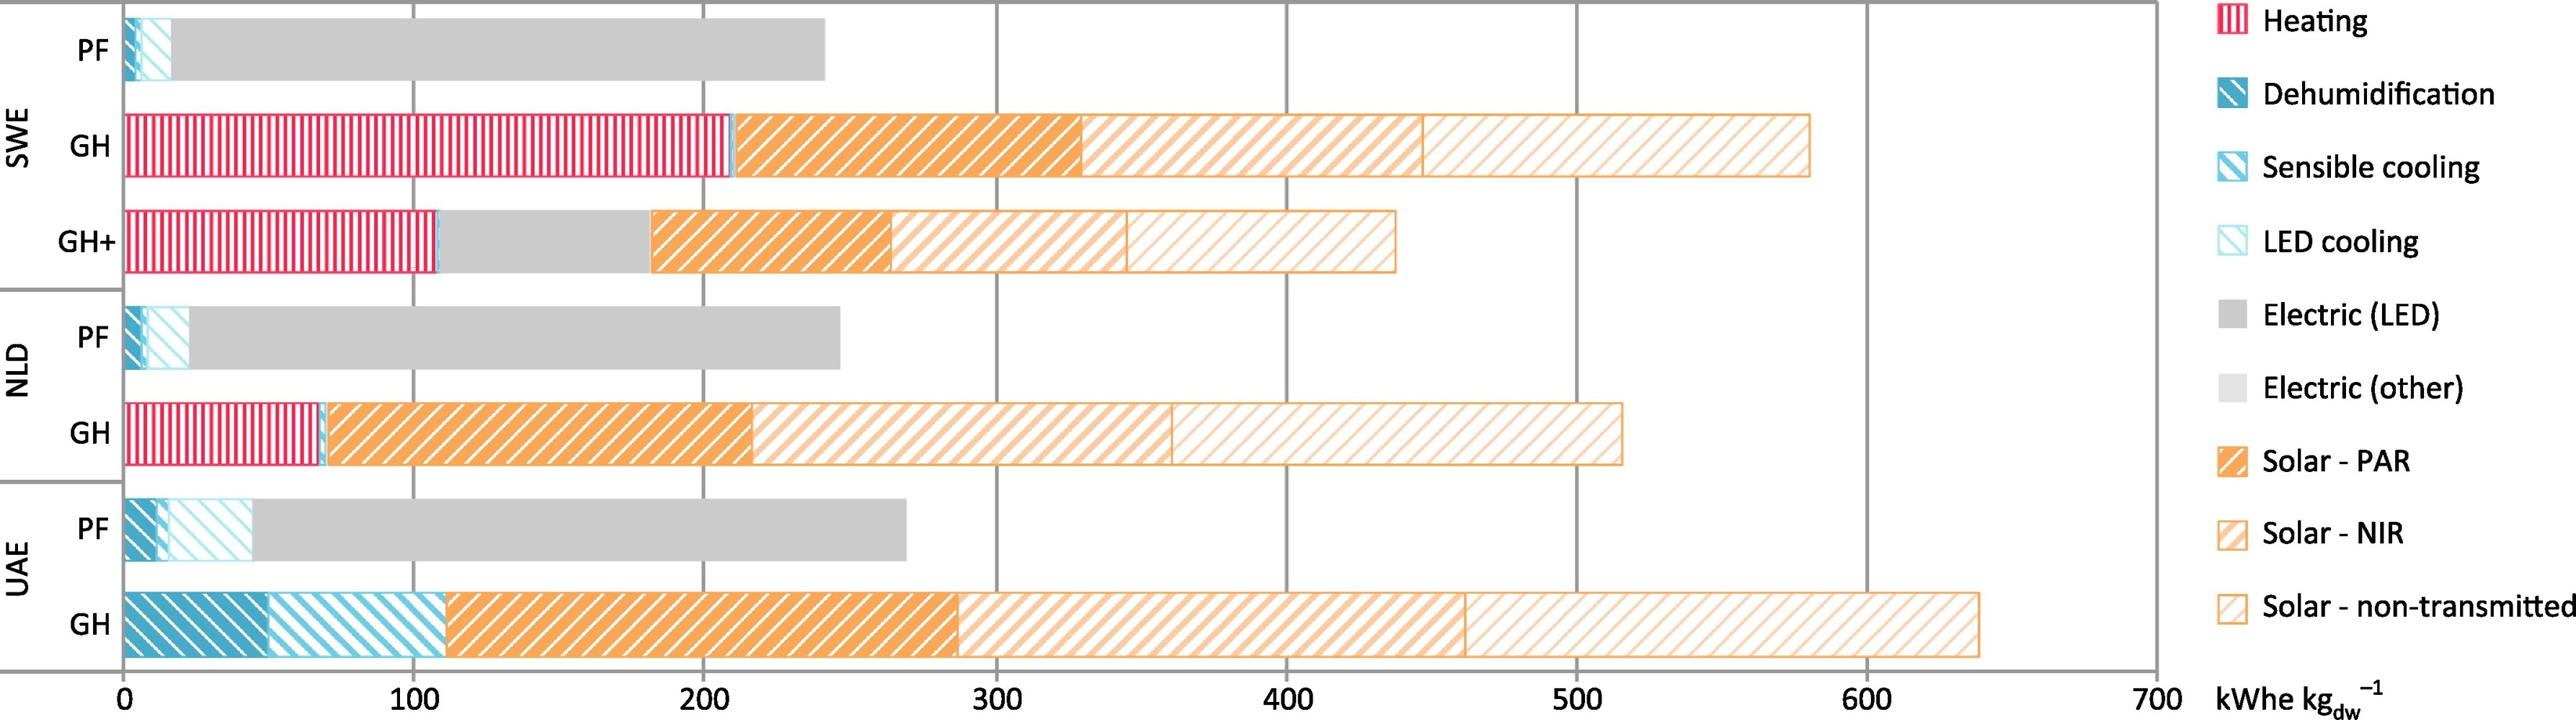
\includegraphics[width=\textwidth]{img/energy-sensitivity.jpg}
\end{figure}
We focus on the bars labeled PF, for plant factory.
In contrast, GH stands for greenhouse.
These farming methods were analyzed for Sweden (SWE), Netherlands (NLD) and the United Arab Emirates (UAE).
We will look closer at the Dutch data, since the climate is the closest to Germany.
As we can see the vast majority of electricity is used for illumination by \acp{led}.
The cooling for this lighting system comes in second and third is dehumidification.
Cooling and dehumidification are the realm of atmosphere control.
Irrigation is not considered in this study.

% https://doi.org/10.1016/j.applthermaleng.2023.122129
Another study @arcasi2024 analyzes the sensitivity for different amounts of lighting and temperatures.
Copenhagen and Naples were the closest locations to Germany examined in this paper.
They come to a similar conclusion as illumination consumed between 65 to \SI{85}{\percent} of electricity.
10 to \SI{20}{\percent} can be attributed to \ac{hvac} systems.
Once again electricity use of irrigation was not considered in this study.
However, a whitepaper by the Association of Vertical Farming @zeidler2017 and anecdotal data for example from iFarm suggests that the consumption is negligible.
They find that illumination together with air management make up 95 to \SI{98}{\percent} of the total energy demand of vertical farming systems.
% https://ifarm.fi/blog/how-much-electricity-does-a-vertical-farm-consume
In the further analysis, it is assumed to be inconsequential.

This knowledge now determines the main design choice of the conceptualization.
Illumination is by far the biggest contributor to electricity need and so natural lighting shall be used.
Now one could argue that a vertical farm like this would offer no advantage over traditional greenhouse cultivation.
However when looking at the energy consumption data for greenhouses (GH) in the Netherlands (NLD) shown in figure \ref{fig:energy-sensitivity}, we can see that the power demand largely originates from heating.
The solar energy is supplied by the sun and does not need to be taken into account.
High power draw from heating makes sense in a greenhouse context.
The advantage of this cultivation method is to extend the growing season.
So in colder months it needs to be kept warm artificially.
However, a greenhouse is surrounded by badly insulated glass.
Furthermore, it has a wide interface for heat loss to the ground.
When placing the farm on the side of buildings, a distinct advantage emerges.
One of the big outside surfaces is no longer exposed to heat loss.
Instead, the building now provides heat gain to the farm.
Room temperatures humans are comfortable with are usually around 18 to \SI{21}{\degreeCelsius}.
Higher than what lettuce needs to grow.
The effectiveness of this will be shown later in the \nameref{chap:simulation}.
% More on the plants' specific temperature requirements can be found in the next section.
The interface for heat loss to the ground is minimized as well.
And of course other advantages like more regional production -- right inside the city -- remain.
% This knowledge now justifies one of the main design choices made in the conceptualization.
% To use 
Next, the factors influencing yield will be examined.
This will determine what subsystem shall retain optimal control and which will be no focus of this work.

\subsubsection{Yield Analysis}
\label{subsub:yield-analysis}
With the yield analysis we want to find out which input will produce the biggest difference in plant production.
As mentioned before irrigation is a solved problem and this system is assumed to provide water and nutrients in an optimum manner.
We will go off of a lettuce model to see which inputs the system deems important.
The inputs are air temperature, CO$_2$ concentration and \acl{par}.
It is difficult to make consistent statements about the influence of the parameters.
Since the optima change for different combinations of inputs.

When examining yield, we first need a definition of what is meant by that.
It depends largely on the crop under investigation.
The fruiting body, roots, leaves or even whole plants can all be considered produce in different contexts.
As argued before, we chose lettuce as our crop.
For this food item, basically the whole plant can be sold and so yield will be roughly equivalent to weight.
The yield model implemented in the later chapters was first proposed by @van\_henten1994.
It measures yield by modelling dry weight of the plant.
For this, mass is split up into the state variables structural $x_{sdw}$ and non-structural dry weight $x_{nsdw}$.
The model is composed of two nonlinear ordinary differential equations.
The development of these two state variables is given by
\begin{align*}
  % \begin{equation*}
  \frac{\mathrm{d}x_{nsdw}}{\mathrm{d}t} &= c_\alpha f_{phot} - r_{gr} x_{sdw} - f_{resp} - \frac{1-c_\beta}{c_\beta} r_{gr} x_{sdw}\\
  % \end{equation*}
  % \begin{equation*}
  \frac{\mathrm{d}x_{sdw}}{\mathrm{d}t} &= r_{gr} x_{sdw}
  % \end{equation*}
\end{align*}
with parameters $c_\alpha$ (-) being the conversion rate of CO$_2$ to CH$_2$O and $c_\beta$ (-) representing the yield factor.
$f_{phot}$ (\si{\g\per\square\m\per\s}) describes gross canopy photosynthesis, $f_{resp}$ (\si{\g\per\square\m\per\s}) the maintenance respiration and $r_{gr}$ (\si{\per\s}) the specific growth rate.
% They describe the development of these two state variables in accordance to the inputs.
The whole model is too extensive to be shown in this section and so only the top level equations are presented here.
What is important for the investigation at hand are the dynamic inputs which influence this model.
These are air temperature, CO$_2$ concentration and \acl{par}.
In the implementation \ref{subsub:yield-model} the whole model can be seen.
% For a more detailed discussion, please refer to the original paper.

There are two ways to gain more information about a system.
Running experiments in real life and simulating the system with a model.
@van\_henten1994b followed up with a sensitivity analysis of the proposed model.
They found that radiation has the highest influence very closely followed by CO$_2$ concentration.

We choose one crop to optimize, however it is assumed that similar dynamics also play a role in other plant species.
This is important, since this work tries to establish a general system.
It does not aim to overfit to a specific crop type.
This is why the energy impact of existing farms will be weighted more heavily than the yield analysis.

Lettuce is chosen for a few different reasons.
Firstly it is well suited to aeroponic cultivation \textcolor{Blue}{needs ref}.
Secondly it grows quickly and consequently is more economically viable as for instance grain crops.
This makes it one of the most used and researched crops in academic and commercial domains alike.
Most of the different varieties of lettuce have similar growing conditions, hence no differentiation is made in this work.

Now that we have a system we want to optimize, we need to analyze it more deeply.
There are two ways this can be accomplished.
Real plants in experiments and models in simulation.

Temperature is a factor we need to control, to achieve an advantage over traditional agriculture.
Otherwise, non-competitive.

\paragraph{Experiments}
For \textit{experiments} we look at available literature.
Some paper suggests light spectrum has an even bigger impact than illumination magnitude.
As discussed in the fundamentals we do not consider altering spectrum however.

\paragraph{Simulations}
For \textit{simulations} we implement a lettuce yield model proposed by Van Henten @van\_henten1994 in Modelica.
The model is a system of nonlinear partial differential equations \textcolor{Blue}{check if actually right}.
A follow-up paper @van\_henten1994b assessed the sensitivity of the input parameters.
Their analysis showed the highest impact for radiation and CO$_2$ concentration.
Radiation displayed slightly more effect on growth.
This is mostly consistent with the experimental data discussed above.

% Following the usual procedure in control theory, it would be best to linearize the system.
% For linear control systems the methods are far more developed.
% This is usually done when we have one operating point the system shall be kept in, limiting the linearization error.
% However, our system shall grow, so we do not have a stable operating point.

% Next plants are quite slow systems in the technical context.
% Dynamics with a slow response and high dead time are generally not well suited to the methods of control theory \textcolor{Blue}{needs ref}.
% This is why we will analyze the plant model with a more crude but still effective approach.

% The specifics are discussed later in chapter \ref{chap:simulation}.
% For now only the inputs and outputs are considered.

\textcolor{Blue}{Instert picture of plant model.}

Water and nutrient delivery is mostly a solved problem in moderate climates and specifically \ac{cea} contexts.
Hence, it does not play a role in the yield calculation.
The properties of interest in the atmosphere are temperature $u_T$ and CO$_2$ concentration $u_{CO2}$.
For illumination, \ac{par} $u_par$ is considered.
As is convention in control settings, inputs are labeled with $u$ and outputs with $y$.



Plants come in a variety of different forms and varieties.
Lettuce is chosen because it is the most researched in the field.
To judge crop yield, which factors are important.
We present a yield 

To be able to judge which factors influence plant yield, we need
As @esmaili2020 showed, highest variance for lighting, suggesting most impact to yield.

To minimize energy consumption we have already found above 
Lighting provides the biggest leverage.
This was a priority when designing the system.
Similar to greenhouse cultivation, natural light shall be used.
But what impact does this have on insulation potential and maximizing yield.
For insulation there is none.

Let us analyze what elements enable us to maximize yield.
Yield is produced by the plant, so let 
For this we will introduce the Yield model for lettuce.
\textcolor{Blue}{Input block diagram plant model and interactions.}

Water and nutrient delivery is mostly a solved problem.
This is why it is not taken as an input to the yield model.
We will deploy an aeroponics system as reasoned in the fundamentals \ref{sub:fund-cea-irr}.

The Energy Analysis \ref{subsub:energy-analysis} has shown that illumination in this context takes the highest amount of resources.
The optimal lighting conditions can be achieved with reasonable complexity increase.
One reason to optimize the lighting.

For the atmospheric conditions
For greenhouses, common practice is to elevate levels but keep windows open.
As this work is in the context of sustainability, it is not considered supplementing CO$_2$.

From the first point we can deduct t

We will define this by the functions the system needs to provide.

So what exactly is it this work tries to achieve and what are relevant properties?
On a high level
This work wants to demonstrate the feasibility of a system.
This work wants to advocate, that greening the future city environment and making food production more resilient and better for the climate can be combined.
It shall be determined if it makes sense to put plants on buildings.
We want to take care of a plant.

The plant is a system we can not control directly.
However, indirectly there exists significant potential to optimize the plant environment.

Define plant system.

Definition System.
To understand what is needed of a system we first need to define its boundaries.
And interactions with adjacent systems.
Context in which it is situated.
Define scope which we can control.

Yield model highly nonlinear.
Difficult to analyze.
Additionally, very slow systems with dead time basically impossible to control via classic control theory \textcolor{Blue}{needs ref}.

For humidity / vpd, there could be no data found comparing the sensitivity to the other parameters.
It is assumed that enough air exchange will happen from the farm to the outside air to achieve reasonable growth.
This is what happens in greenhouses anyway.

\subsection{Conclusions from the analysis}
\label{sub:conc-analysis}
The energy analysis showed that we need to focus on the lighting for minimizing energy.
As a result natural lighting will be utilized.
From the yield analysis the result was that again we need to focus on the lighting.
As a result we provide a lighting system for the farm to supply optimal \ac{dli} to the crop.
Additionally as \ac{hvac} systems are expensive compared to \acp{led} -- another reason to not focus on atmosphere control for now.

The last section defined the system in question clearly.
It showed the most impactful parts.
With this knowledge, we can prune the system description to arrive at our concept.
It is pretty similar to the system design proposed before but now only showing the parts which actually will be implemented.
The atmosphere control will no longer distinguish between the mass flows of different elements.
Instead, we accumulate them together to the mass flow $\dot{m}_{Air}$.
As we also do not consider control for the air temperature, we remove the heat flow from the atmosphere control.



\section{General Concept}
\label{sec:concept}
From \ref{}, we have a clear picture on the electrical and control systems necessary.
However, for a complete implementation some secondary functions need to be fulfilled.
For example an atmosphere control absent an envelope to keep the air in, hardly makes any sense.
Additionally, we need to supply energy to the systems and provide a structure to mount everything.
From the chosen crop -- lettuce -- there also follows a high turnover rate.
It is usually ready in four to six weeks.
Therefore, easy mount and demount necessary.
These supporting components to the system as well as the tasks of the main system will be formalized and presented in the next section as functions.

\subsection{Functional Architecture}
\label{sub:func-arch}
Definition of our scope, extracted from the analysis.
The functions our concept shall serve, breaking down the goals of minimizing energy consumption and maximizing yield.
\begin{itemize}
	\item Supply optimal lighting conditions.
	\item Provide a reasonable temperature range to grow lettuce.
	\item Maintain sufficient air exchange to keep CO$_2$ and humidity levels in check.
	\item Sustain optimal water and nutrient delivery.
	\item Serve a mounting structure to be able to retrofit the system onto buildings.
	\item Provide transportation mechanism to easily harvest and replant the crops.

\end{itemize}

Defining what is out of scope makes it easier to understand.
Functions which shall \textbf{not} be implemented.
\begin{itemize}
	\item Provide optimal CO$_2$ concentration.
	\item Provide optimal temperatures.
	\item Provide optimal light spectrum.
	\item Provide optimal humidity levels.
	\item Provide .

\end{itemize}

Now that we have gathered an understanding of the system and the scope that this work targets.

Energy system does not serve a particular function.
It is a secondary function enabling the functioning of the other functions.

Water tanks to store water.
Pumps can run during the day when solar output available.

\subsection{Structural Architecture}
\label{sub:stru-arch}
SysML offers a standardized way to convey system information.
It offers an informational model as well as a visual representation for systems engineering.
Therefore, it will be used to present the concept.
There are different diagram types, structural diagrams are used.
More specifically the \ac{ibd} is used.
This type is taken to describe a systems constituents.
The different parts are pictured by rectangles.
Connections have a diamond shape on the part which is deconstructed into its constituents.
The arrow points to the components.
For a full system design, there are a myriad of diagram types to be used in SysML.
However, this work will not concretize to deeply and therefore only use this one diagram type.
This will enable us to describe the proposed system.
From the main system description and the other secondary functions the system needs to provide, we can now extract the structural architecture more easily.

For the structural architecture we will go off of two things we developed so far.
Firstly the main system from our system definition (\ref{}).
Secondly the functional architecture with all the systems needed to support the functioning of the main system.
This distinction is a little bit arbitrary but needs to be made at some cut-off point.
For example the system description could include a system for planting and harvesting, since it is technically needed to convert the plant to economic output.
However, the system description grows to large for this work in this way.
And so main functions and supporting functions are distinguished.
The order these will be introduced roughly follows a spatial line starting from the building and attaching the systems going outward to the city.
For comprehensibility’s sake, we will present the architecture going spatially from the building to the outside.
This will be represented with more foundational components to the left of the diagram.
The introduction of these blocks will follow a particular pattern.
First the function of the block is presented, then requirements laid out and then the structure of the subsystem is presented in written and visual form.
If useful a 3d model is presented to visualize the architecture with a tangible example.

% Also, a 3d model is presented to make the architecture more tangible.
Following the theme of going from the building further outside, let us first get a look at the building in question.
It can be seen in \ref{fig:3d-building}.
The pictures of the building faces were made by the author.
The 2d plane the model sits on was taken from a satellite image in Google Maps \textcolor{Blue}{am I allowed to do this?}.
The 3d geometry data is taken from \textcolor{Blue}{needs ref}.
\begin{figure}[htbp]
  \centering
  \caption{3d model of the EEI-tower.}
  \label{fig:3d-building}
  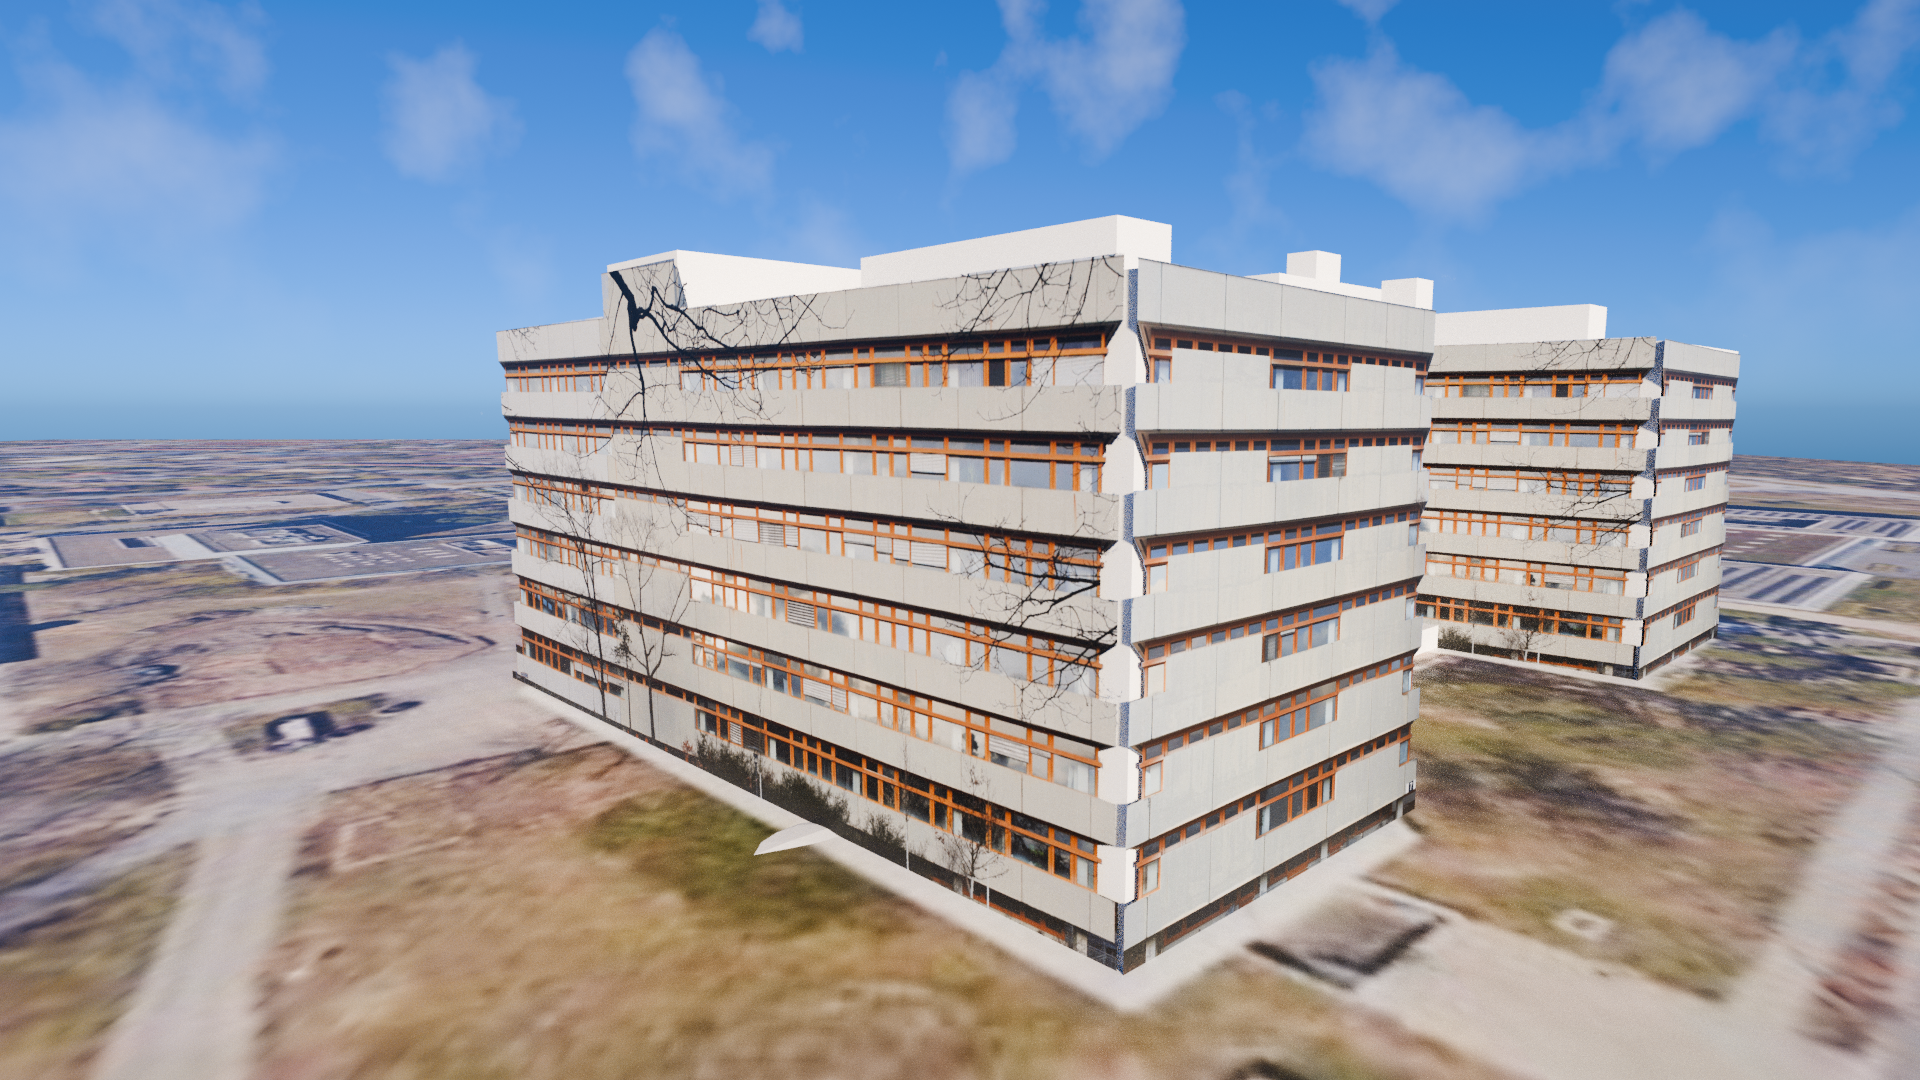
\includegraphics[width=\textwidth]{img/3d_model/building.png}
\end{figure}

\subsubsection{Load-Bearing Structure}
\begin{wrapfigure}{R}{0.4\textwidth}
	\caption{The load bearing structure.}
	\label{wfig:load}
	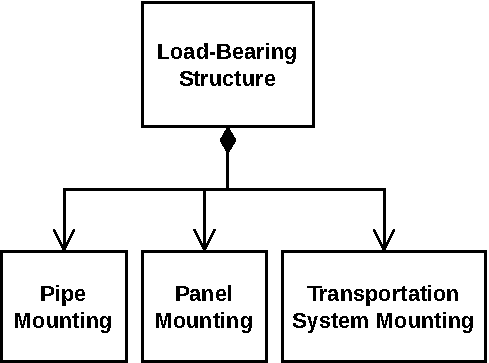
\includegraphics[width=0.4\textwidth]{img/architecture/load.pdf}
\end{wrapfigure} 
With this in mind, let us first discuss the mounting structure.
Its function is to provide a load bearing foundation for any other subsystem to attach to.
One point to note is that the system shall be retrofitted to existing buildings.
Therefore, it should be self-contained in supporting its own weight.
Building faces are very diverse, so it should be independent of the present structure.
Of course, it needs to be closely matched to the existing building because the panels are only mounted on the facade.
The mounting provides the interface for other subsystems.
% These are defined later.
The pipes, panels and transportation system are part of different components and are defined later.
\textcolor{Blue}{Need to fit to presentation pattern.}
% Pipes are for the bigger water system, Panels represent basically the root environment and its direct control with irrigation.
% The transport system 
% It shall not damage the facade or other structures on the existing buildings.

\subsubsection{Water System}
\begin{wrapfigure}{R}{0.6\textwidth}
	\caption{The water system mixing and delivering the nutrient mix.}
	\label{wfig:water}
	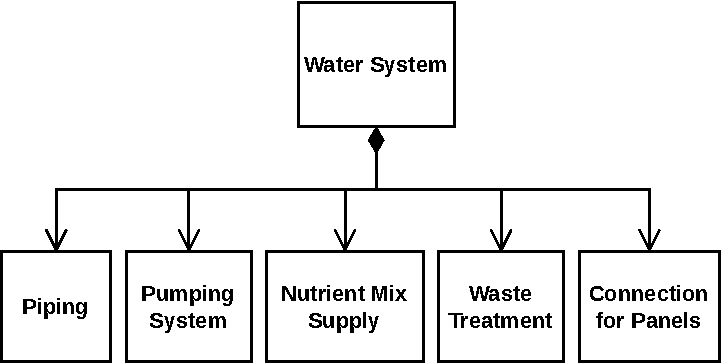
\includegraphics[width=0.6\textwidth]{img/architecture/water.pdf}
\end{wrapfigure} 
The next system that would need to be installed is the water system.
It does not have a direct equivalent in our system description from \ref{}.
There we already presupposed the water and nutrient mix to be prepared and available to the irrigation system.
The water system will take care of this task.
Preparing the nutrient mix and optimal \ac{ec} and pH-levels.
This mixture is then supplied to the panels.
It needs to interface to the actual irrigation system illustrated by the component 'connection for panels'.
As discussed later we will also utilize a solar array.
It makes sense to pump the water during the day up to a water storage on the roof of the building.
During nighttime gravity will provide water pressure to the system.
A connection to the water system of the building is also conceivable.
To keep the retrofit concept minimally invasive though, a separate water circuit is proposed here.
\textcolor{Blue}{Need to fit to presentation pattern.}

\subsubsection{Plant Panels}
For the actual irrigation system, we will go into a little bit more depth.
As a general concept, they are chosen to modularize the whole system.
Providing a standardized platform for any building.
One could imagine around three different sizes to best accommodate the space available on the facade.
Additionally, they provide smaller compartments to take care of.
This is important as discussed before to stop the spread of plant diseases.
As well as providing fine-grained control of the plants.
Ideally you would want a control system taking care of every plant individually.
This however entails high cost and a trade-off needs to be made similar to the lessening of automation in \ac{cea}.
The modularization makes it possible to stagger planting and harvesting.
Now that we have a rough outline of what we want the system to look like -- the framework -- we can take a closer look at how and what shall be implemented.
As discussed before, the panels shall take the role of irrigation.
For this they need to provide a closed volume for the root zone.
This is the main structure of the presented panels.
As detailed in \ref{sub:fund-cea-irr} the system will use aeroponics.
This of course can be exchanged for any other hydroponic strategy inside the panels.
For example one could imagine \ac{nft} channels inside the same panels in which the plant roots reside.
For the aeroponic system, a ultrasonic piezoelectric vaporizer is placed in a water filled upper part of the panel.
This sustains a fog holding moisture and nutrients inside the root environment.
This technology of course is not perfect.
Anecdotal information suggests that these vaporizers will crust up with salts dissolved in the water over time.
They also heat up the root zone.
Root zone temperature is considered separately from the main air temperatures in some studies.
Suggesting that it might be an impactful parameter in plant growth and health.
This work did not analyze this further though as the general concept of the panel can be the platform for different irrigation strategies.
The root volume is controlled according to the system design with a feedback control.
A humidity and temperature sensor supplies the \ac{vpd} information to a controller.
The panel should also be able to get rid of the waste products exuded by the plant root.
An outflow is provided by the concept.
The panel structure holds all the different parts interacting with each other.
The 3d model exemplifing this idea can be seen in figure \ref{fig:3d-panels}.
\textcolor{Blue}{Need to fit to presentation pattern.}
\begin{figure}[htbp]
  \centering
  \caption{The plant panels proposed by this work.}
  \label{fig:panels}
  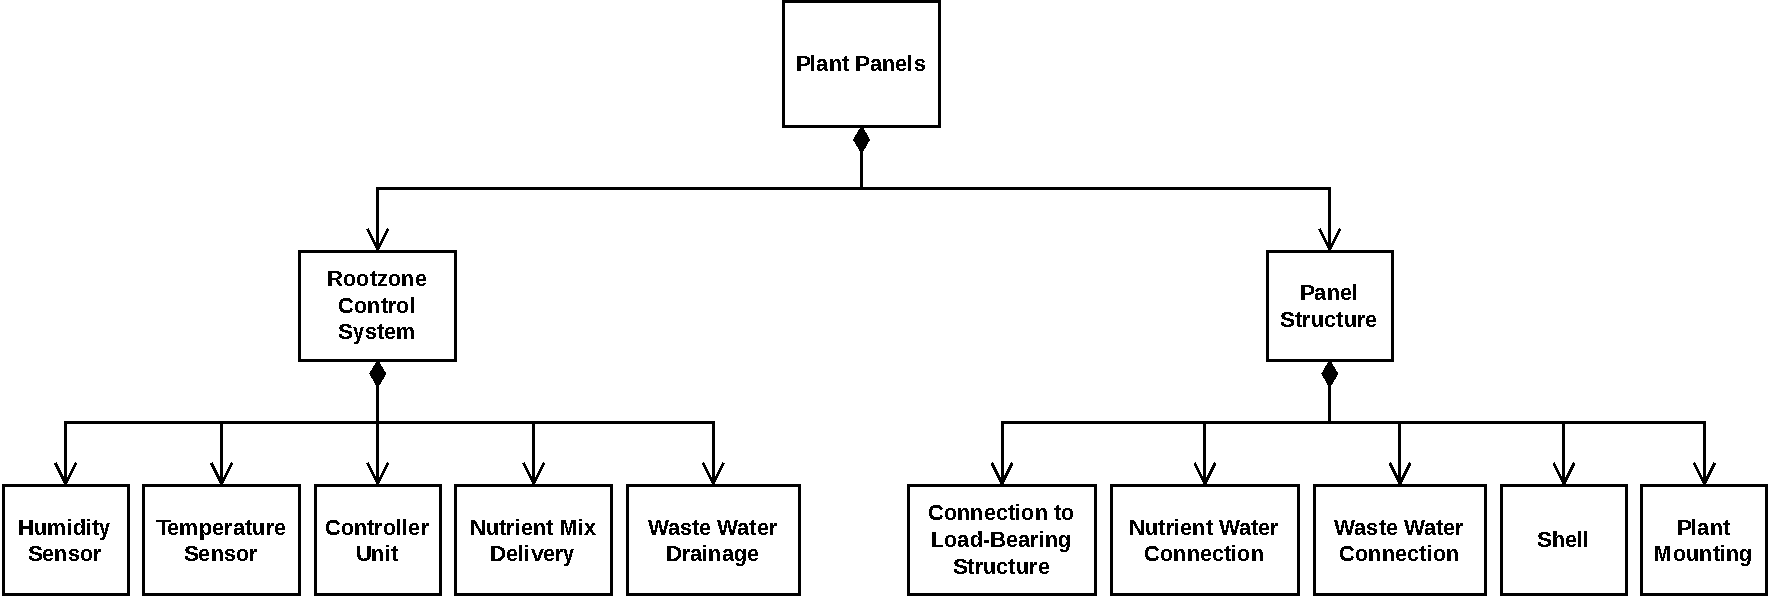
\includegraphics[width=\textwidth]{img/architecture/panels.pdf}
\end{figure}

\begin{figure}[htbp]
  \centering
  \caption{3d model showing the plant panels mounted to the building facade.}
  \label{fig:3d-panels}
  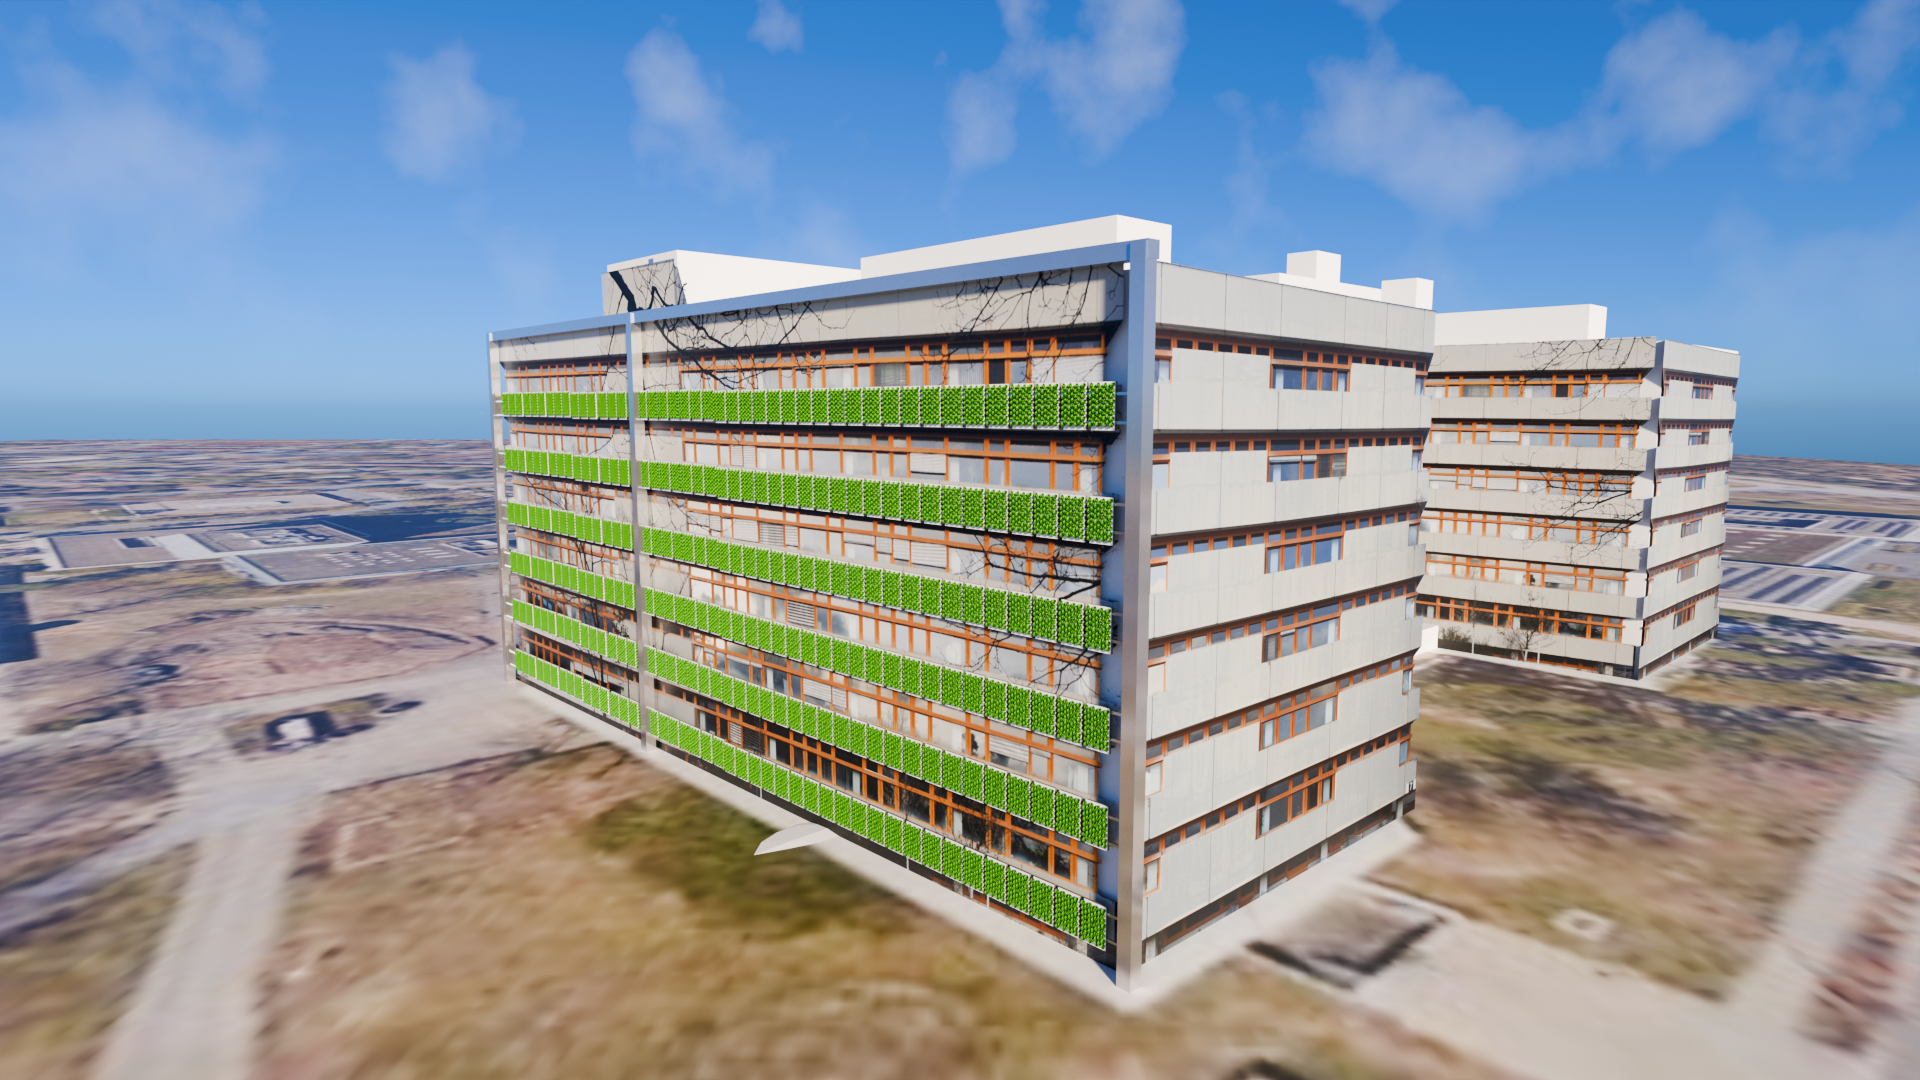
\includegraphics[width=\textwidth]{img/3d_model/3d-3-panels.png}
\end{figure}

\subsubsection{Transportation System}
\begin{wrapfigure}{R}{0.5\textwidth}
	\caption{The transport platform eliminating the need for manual (de-)mounting.}
	\label{wfig:transport}
	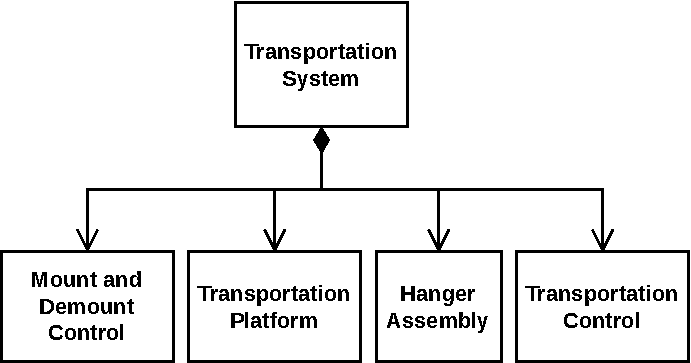
\includegraphics[width=0.5\textwidth]{img/architecture/transport.pdf}
\end{wrapfigure} 
As mentioned before the system needs to transport the panels to and from the facade.
This is again a supporting function not found in the main system description.
The system needs to mount and demount the panels to and from the load bearing structure (\ref{wfig:load}).
Then it needs to move the panels across the face of the building to a base where they can be harvested and restocked with fresh plant shoots.
It should also be as low profile as possible.
From this the concept of a wire-hung platform is developed.
It consists of a main 'platform' responsible for (un-)loading the panels and necessary 'control'.
A 'hanger assembly' made up of steel wires moves the platform.
The structural architecture of the block can be seen in figure \ref{wfig:transport} while a closeup of the transportation system is shown in picture \ref{fig:3d-transport}.

\begin{figure}[htbp]
  \centering
  \caption{3d model showing the general idea of the transport platform.}
  \label{fig:3d-transport}
  \includegraphics[width=\textwidth]{img/3d_model/3d-4-transport-closeup.png}
\end{figure}

\subsubsection{Energy System}
Next a system needs to provide power to all the electronic subsystems.
This can be expanded into energy storage and generation as well.
The reason for this is to counteract the energetic impact generated by the farm as much as possible.
This is done because as mentioned before, the German electricity mix is far from carbon-neutral.
Consistent with our motivation to make food production more green, a solar array is considered to generate energy.
As we will show later in \ref{chap:simulation} it may even be possible to completely nullify the energy consumption with this procedure.
Requirements.
Provide a \ac{dc} power circuit to all the components.
The biggest consumer of power, the \acp{led} need \ac{dc} and therefore the main circuit is chosen to be \ac{dc}.
This fits in well with a battery and solar array.
Next the system shall generate energy by a solar array.
The reasons for this are mentioned above.
The chosen irrigation strategy is highly dependent on active control, otherwise the plant roots dry out quickly.
So we need to store energy to be resilient to power outages.
The system shall provide a connection to the grid.
This is because the energy generation and consumption in our farm show a negative correlation.
When the sun is shining, the \ac{pv} installation will provide a lot of energy, while not much energy is needed for supplemental lighting.
Conversely, when there is little sun, we have a high energy demand from the \acp{led}, while not much energy is generated.
Structure.
So from these requirements we separate the system into the three parts 'energy generation', 'energy storage' and 'energy distribution'with appropriate parts in each seen in figure \ref{fig:energy}.

\begin{figure}[htbp]
  \centering
  \caption{The energy subsystem.}
  \label{fig:energy}
  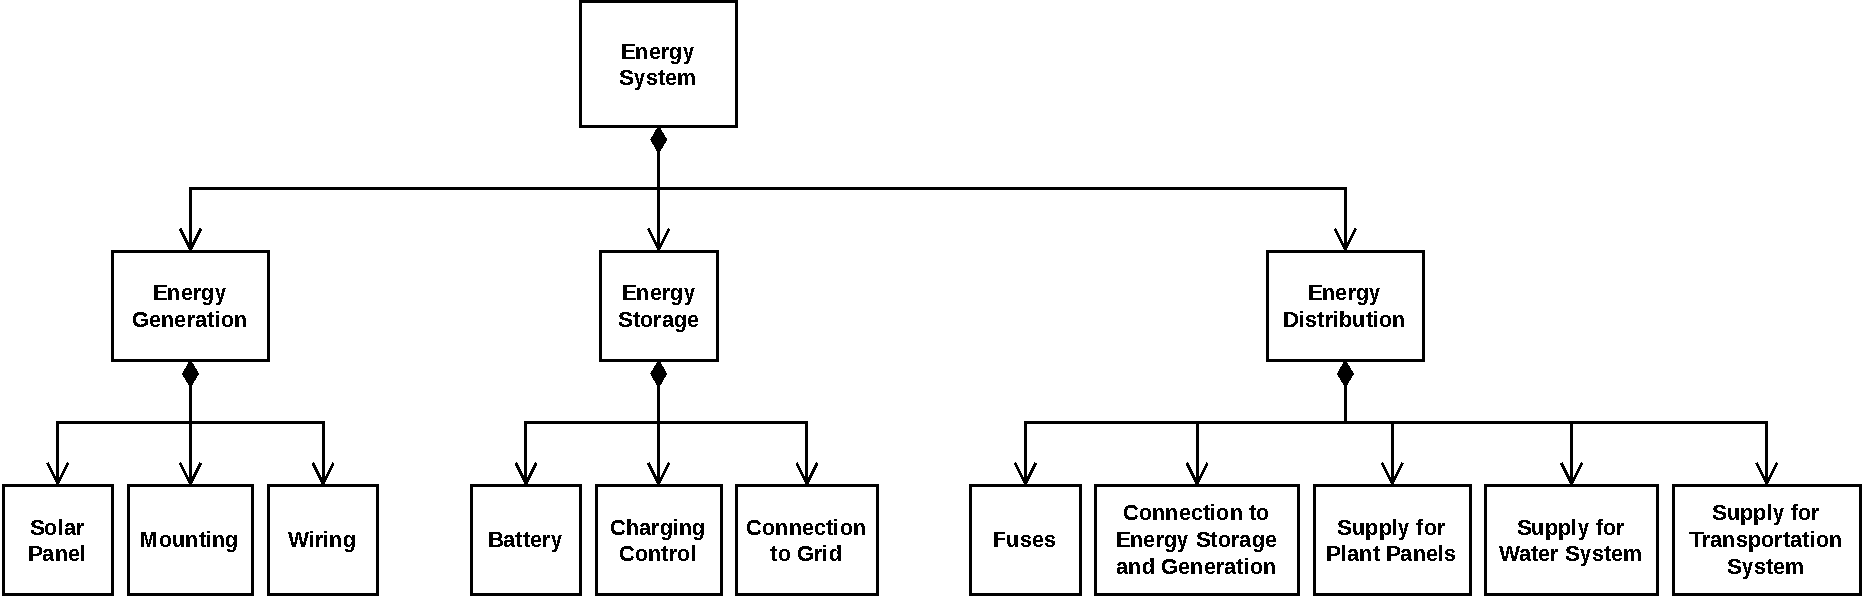
\includegraphics[width=\textwidth]{img/architecture/energy.pdf}
\end{figure}

\subsubsection{Climate Control}
The function of optimal light and reasonable atmosphere control is compounded into one part, the climate control.
Requirements and structure.
The lighting system as discussed before needs to provide a structure to shade from excessive light.
This is proposed to be simple semi-transparent cloth similar to existing greenhouses.
It would be deployed similar to an awning to not block the view of the people inside the building.
Next if there happens to be little sun, we need to supply supplemental lighting.
\acp{led} are chosen for a few reasons.
Their spectrum can be adjusted for the task of growing plants quite well.
They are comparatively cheap and efficient and therefore also do not produce a high amount of excess heat.
The amount of light entering the farm needs to be monitored and the shades and \acp{led} regulated with a control system.

For the atmosphere control we need to monitor the air volume and so sensors specified in section \ref{subsub:engineered-system} are employed.
Ventilation is required.
This takes the form of a passive system in our concept.
Simple windows at the top and bottom of the farm will provide airflow.
They can be controlled according to the sensor inputs.
\textcolor{Blue}{What do I do with dehumidification?}
The internal block diagram can be seen in figure \ref{fig:climate}.

\begin{figure}[htbp]
  \centering
  \caption{The climate control to take care of the leaf environment.}
  \label{fig:climate}
  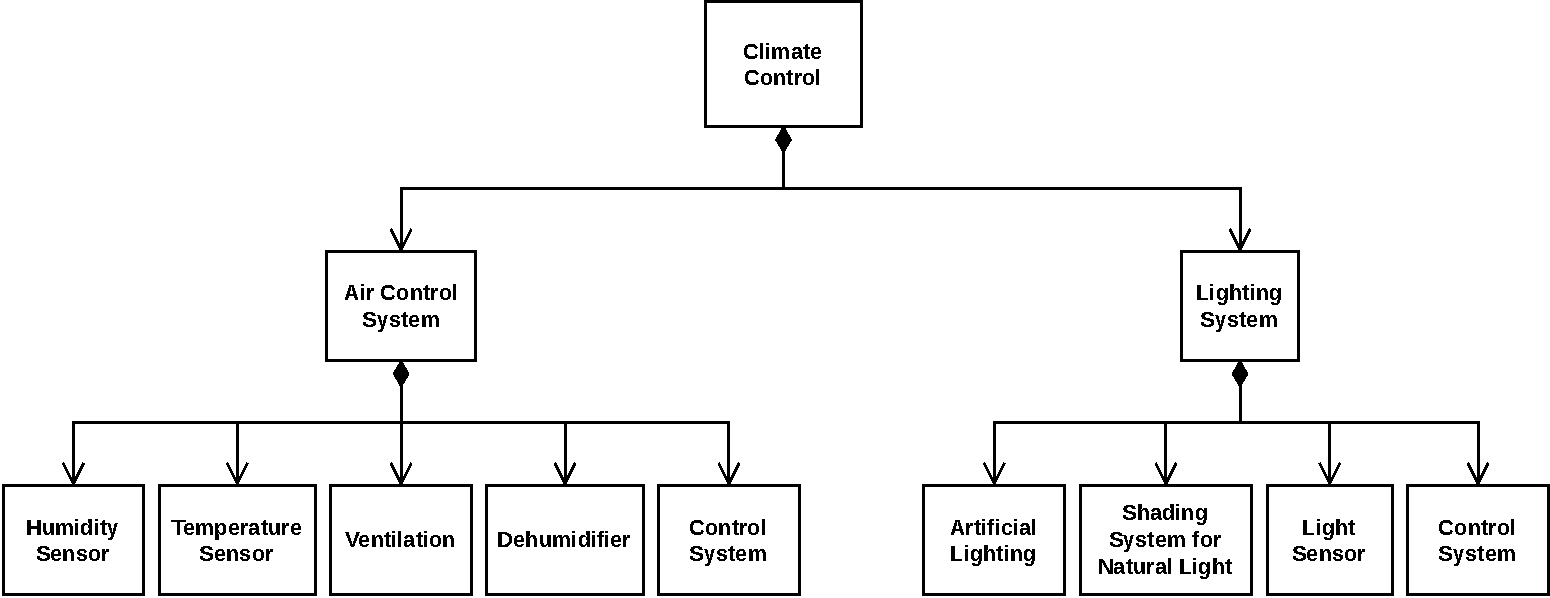
\includegraphics[width=\textwidth]{img/architecture/climate.pdf}
\end{figure}

\subsubsection{Envelope}
\begin{wrapfigure}{R}{0.3\textwidth}
	\caption{The envelope segregating the farm from the city environment.}
	\label{wfig:envelope}
	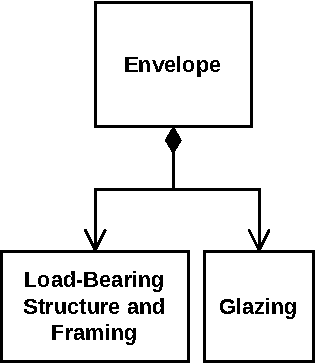
\includegraphics[width=0.3\textwidth]{img/architecture/envelope.pdf}
\end{wrapfigure} 
The envelope provides the secondary function of separating the farm from its surroundings.
This is not formulated explicitly in the functions above.
Because it is inherent to have a separate environment if you would like to provide atmosphere control.
% This is quite primary as otherwise no \acl{cea} is possible.
Requirements and structure.
As the function says the envelope needs to provide a separation to the city environment.
This is accomplished by self-supporting framing and some sort of glazing.
For this work we propose glass as it is durable and visually pleasing.
This is wrapped around the whole farm and building.
Not a requirement for our concept but another resulting function of this structure is the insulation.
One could imagine confining the envelope to the panels and therefore facade area.
When just covering the facade it would be best to separate the envelope and the insulation into two distinct parts.
This is because traditional insulation needs to be very close to the wall with little air movement.
For this work we chose to simplify this structure and therefore just encapsulate the building in a greenhouse shell.
This comes with the added benefit of insulating the window area of the building, which usually is responsible for a high fraction of the heat loss of a building.
The complete architecture can be seen in figure \ref{fig:architecture}.
It is cut-off at the second level of block definition, as otherwise it would become too unwieldy to present whole.

\begin{figure}[htbp]
  \centering
  \caption{The structural architecture of our farming concept.}
  \label{fig:architecture}
  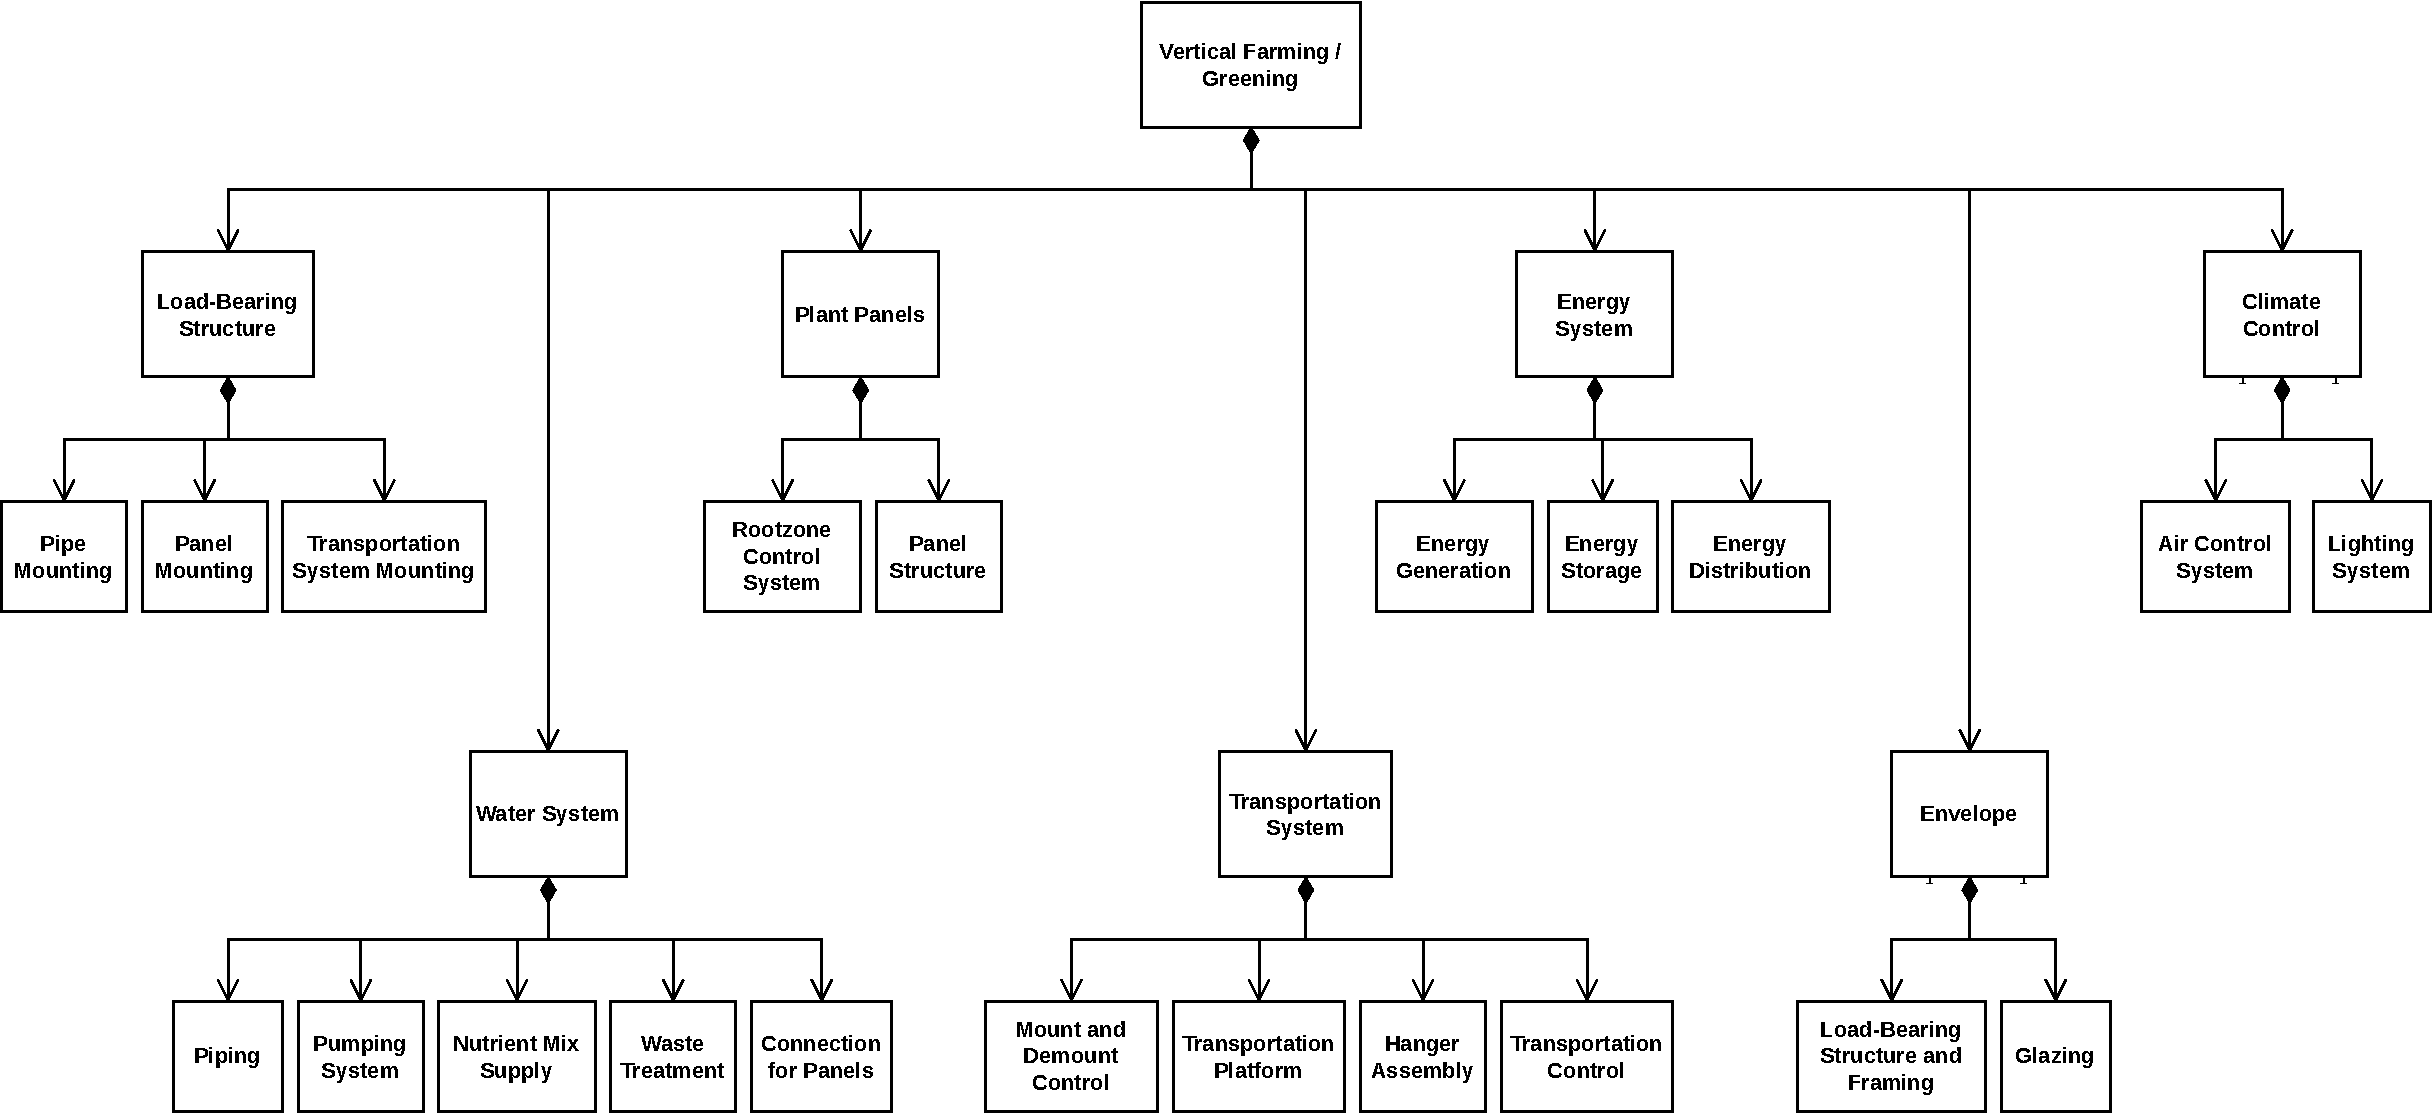
\includegraphics[width=\textwidth]{img/architecture/architecture.pdf}
\end{figure}
\textcolor{Blue}{Switch climate control and envelope in full architecture.}

\section{Feasibility}
\label{sec:feasibility}
Lastly to judge the proposed system a number of metrics are introduced.
These serve to evaluate the feasibility of the concept.
Feasibility in this work does not mean that a system like this definitely makes sense.
But only to judge and evaluate the concept on a few different fronts.
% Metrics to evalute feasibility of the concept:
The metrics this work proposes, are as follows:
\begin{itemize}
	\item The energy consumption can be met through a solar installation covering at most the area on the roof.
	\item Yield can offset investment costs in a reasonable timeframe.
	\item Farm provides measurable insulation increase in comparison with the 'naked' building.
	\item Acceptance of potential customers to put a greenhouse on the side of their buildings (not evaluated in this work)
\end{itemize}
These points will be picked up later in \ref{chap:results} to assess the outcomes of this work.

\section{Energy System Architecture}
\label{sec:architecture}

\subsection{Choice of Components}

Shading is not considered in this work to preserve visibility from the building to the outside.
And so natural radiation $R_\text{N}$ shines unimpeded onto the plant.
Considering the importance of illumination to the growth of the plant however, this might need be revisited in future works.

Trace substance.
